
% Default to the notebook output style

    


% Inherit from the specified cell style.




    
\documentclass{article}

    
    
    \usepackage{graphicx} % Used to insert images
    \usepackage{adjustbox} % Used to constrain images to a maximum size 
    \usepackage{color} % Allow colors to be defined
    \usepackage{enumerate} % Needed for markdown enumerations to work
    \usepackage{geometry} % Used to adjust the document margins
    \usepackage{amsmath} % Equations
    \usepackage{amssymb} % Equations
    \usepackage{eurosym} % defines \euro
    \usepackage[mathletters]{ucs} % Extended unicode (utf-8) support
    \usepackage[utf8x]{inputenc} % Allow utf-8 characters in the tex document
    \usepackage{fancyvrb} % verbatim replacement that allows latex
    \usepackage{grffile} % extends the file name processing of package graphics 
                         % to support a larger range 
    % The hyperref package gives us a pdf with properly built
    % internal navigation ('pdf bookmarks' for the table of contents,
    % internal cross-reference links, web links for URLs, etc.)
    \usepackage{hyperref}
    \usepackage{longtable} % longtable support required by pandoc >1.10
    \usepackage{booktabs}  % table support for pandoc > 1.12.2
    

    
    
    \definecolor{orange}{cmyk}{0,0.4,0.8,0.2}
    \definecolor{darkorange}{rgb}{.71,0.21,0.01}
    \definecolor{darkgreen}{rgb}{.12,.54,.11}
    \definecolor{myteal}{rgb}{.26, .44, .56}
    \definecolor{gray}{gray}{0.45}
    \definecolor{lightgray}{gray}{.95}
    \definecolor{mediumgray}{gray}{.8}
    \definecolor{inputbackground}{rgb}{.95, .95, .85}
    \definecolor{outputbackground}{rgb}{.95, .95, .95}
    \definecolor{traceback}{rgb}{1, .95, .95}
    % ansi colors
    \definecolor{red}{rgb}{.6,0,0}
    \definecolor{green}{rgb}{0,.65,0}
    \definecolor{brown}{rgb}{0.6,0.6,0}
    \definecolor{blue}{rgb}{0,.145,.698}
    \definecolor{purple}{rgb}{.698,.145,.698}
    \definecolor{cyan}{rgb}{0,.698,.698}
    \definecolor{lightgray}{gray}{0.5}
    
    % bright ansi colors
    \definecolor{darkgray}{gray}{0.25}
    \definecolor{lightred}{rgb}{1.0,0.39,0.28}
    \definecolor{lightgreen}{rgb}{0.48,0.99,0.0}
    \definecolor{lightblue}{rgb}{0.53,0.81,0.92}
    \definecolor{lightpurple}{rgb}{0.87,0.63,0.87}
    \definecolor{lightcyan}{rgb}{0.5,1.0,0.83}
    
    % commands and environments needed by pandoc snippets
    % extracted from the output of `pandoc -s`
    \providecommand{\tightlist}{%
      \setlength{\itemsep}{0pt}\setlength{\parskip}{0pt}}
    \DefineVerbatimEnvironment{Highlighting}{Verbatim}{commandchars=\\\{\}}
    % Add ',fontsize=\small' for more characters per line
    \newenvironment{Shaded}{}{}
    \newcommand{\KeywordTok}[1]{\textcolor[rgb]{0.00,0.44,0.13}{\textbf{{#1}}}}
    \newcommand{\DataTypeTok}[1]{\textcolor[rgb]{0.56,0.13,0.00}{{#1}}}
    \newcommand{\DecValTok}[1]{\textcolor[rgb]{0.25,0.63,0.44}{{#1}}}
    \newcommand{\BaseNTok}[1]{\textcolor[rgb]{0.25,0.63,0.44}{{#1}}}
    \newcommand{\FloatTok}[1]{\textcolor[rgb]{0.25,0.63,0.44}{{#1}}}
    \newcommand{\CharTok}[1]{\textcolor[rgb]{0.25,0.44,0.63}{{#1}}}
    \newcommand{\StringTok}[1]{\textcolor[rgb]{0.25,0.44,0.63}{{#1}}}
    \newcommand{\CommentTok}[1]{\textcolor[rgb]{0.38,0.63,0.69}{\textit{{#1}}}}
    \newcommand{\OtherTok}[1]{\textcolor[rgb]{0.00,0.44,0.13}{{#1}}}
    \newcommand{\AlertTok}[1]{\textcolor[rgb]{1.00,0.00,0.00}{\textbf{{#1}}}}
    \newcommand{\FunctionTok}[1]{\textcolor[rgb]{0.02,0.16,0.49}{{#1}}}
    \newcommand{\RegionMarkerTok}[1]{{#1}}
    \newcommand{\ErrorTok}[1]{\textcolor[rgb]{1.00,0.00,0.00}{\textbf{{#1}}}}
    \newcommand{\NormalTok}[1]{{#1}}
    
    % Define a nice break command that doesn't care if a line doesn't already
    % exist.
    \def\br{\hspace*{\fill} \\* }
    % Math Jax compatability definitions
    \def\gt{>}
    \def\lt{<}
    % Document parameters
    \title{M5 Exam Solutions}
    \author{Tanya Sandoval}
    
    
    

    % Pygments definitions
    
\makeatletter
\def\PY@reset{\let\PY@it=\relax \let\PY@bf=\relax%
    \let\PY@ul=\relax \let\PY@tc=\relax%
    \let\PY@bc=\relax \let\PY@ff=\relax}
\def\PY@tok#1{\csname PY@tok@#1\endcsname}
\def\PY@toks#1+{\ifx\relax#1\empty\else%
    \PY@tok{#1}\expandafter\PY@toks\fi}
\def\PY@do#1{\PY@bc{\PY@tc{\PY@ul{%
    \PY@it{\PY@bf{\PY@ff{#1}}}}}}}
\def\PY#1#2{\PY@reset\PY@toks#1+\relax+\PY@do{#2}}

\expandafter\def\csname PY@tok@gd\endcsname{\def\PY@tc##1{\textcolor[rgb]{0.63,0.00,0.00}{##1}}}
\expandafter\def\csname PY@tok@gu\endcsname{\let\PY@bf=\textbf\def\PY@tc##1{\textcolor[rgb]{0.50,0.00,0.50}{##1}}}
\expandafter\def\csname PY@tok@gt\endcsname{\def\PY@tc##1{\textcolor[rgb]{0.00,0.27,0.87}{##1}}}
\expandafter\def\csname PY@tok@gs\endcsname{\let\PY@bf=\textbf}
\expandafter\def\csname PY@tok@gr\endcsname{\def\PY@tc##1{\textcolor[rgb]{1.00,0.00,0.00}{##1}}}
\expandafter\def\csname PY@tok@cm\endcsname{\let\PY@it=\textit\def\PY@tc##1{\textcolor[rgb]{0.25,0.50,0.50}{##1}}}
\expandafter\def\csname PY@tok@vg\endcsname{\def\PY@tc##1{\textcolor[rgb]{0.10,0.09,0.49}{##1}}}
\expandafter\def\csname PY@tok@m\endcsname{\def\PY@tc##1{\textcolor[rgb]{0.40,0.40,0.40}{##1}}}
\expandafter\def\csname PY@tok@mh\endcsname{\def\PY@tc##1{\textcolor[rgb]{0.40,0.40,0.40}{##1}}}
\expandafter\def\csname PY@tok@go\endcsname{\def\PY@tc##1{\textcolor[rgb]{0.53,0.53,0.53}{##1}}}
\expandafter\def\csname PY@tok@ge\endcsname{\let\PY@it=\textit}
\expandafter\def\csname PY@tok@vc\endcsname{\def\PY@tc##1{\textcolor[rgb]{0.10,0.09,0.49}{##1}}}
\expandafter\def\csname PY@tok@il\endcsname{\def\PY@tc##1{\textcolor[rgb]{0.40,0.40,0.40}{##1}}}
\expandafter\def\csname PY@tok@cs\endcsname{\let\PY@it=\textit\def\PY@tc##1{\textcolor[rgb]{0.25,0.50,0.50}{##1}}}
\expandafter\def\csname PY@tok@cp\endcsname{\def\PY@tc##1{\textcolor[rgb]{0.74,0.48,0.00}{##1}}}
\expandafter\def\csname PY@tok@gi\endcsname{\def\PY@tc##1{\textcolor[rgb]{0.00,0.63,0.00}{##1}}}
\expandafter\def\csname PY@tok@gh\endcsname{\let\PY@bf=\textbf\def\PY@tc##1{\textcolor[rgb]{0.00,0.00,0.50}{##1}}}
\expandafter\def\csname PY@tok@ni\endcsname{\let\PY@bf=\textbf\def\PY@tc##1{\textcolor[rgb]{0.60,0.60,0.60}{##1}}}
\expandafter\def\csname PY@tok@nl\endcsname{\def\PY@tc##1{\textcolor[rgb]{0.63,0.63,0.00}{##1}}}
\expandafter\def\csname PY@tok@nn\endcsname{\let\PY@bf=\textbf\def\PY@tc##1{\textcolor[rgb]{0.00,0.00,1.00}{##1}}}
\expandafter\def\csname PY@tok@no\endcsname{\def\PY@tc##1{\textcolor[rgb]{0.53,0.00,0.00}{##1}}}
\expandafter\def\csname PY@tok@na\endcsname{\def\PY@tc##1{\textcolor[rgb]{0.49,0.56,0.16}{##1}}}
\expandafter\def\csname PY@tok@nb\endcsname{\def\PY@tc##1{\textcolor[rgb]{0.00,0.50,0.00}{##1}}}
\expandafter\def\csname PY@tok@nc\endcsname{\let\PY@bf=\textbf\def\PY@tc##1{\textcolor[rgb]{0.00,0.00,1.00}{##1}}}
\expandafter\def\csname PY@tok@nd\endcsname{\def\PY@tc##1{\textcolor[rgb]{0.67,0.13,1.00}{##1}}}
\expandafter\def\csname PY@tok@ne\endcsname{\let\PY@bf=\textbf\def\PY@tc##1{\textcolor[rgb]{0.82,0.25,0.23}{##1}}}
\expandafter\def\csname PY@tok@nf\endcsname{\def\PY@tc##1{\textcolor[rgb]{0.00,0.00,1.00}{##1}}}
\expandafter\def\csname PY@tok@si\endcsname{\let\PY@bf=\textbf\def\PY@tc##1{\textcolor[rgb]{0.73,0.40,0.53}{##1}}}
\expandafter\def\csname PY@tok@s2\endcsname{\def\PY@tc##1{\textcolor[rgb]{0.73,0.13,0.13}{##1}}}
\expandafter\def\csname PY@tok@vi\endcsname{\def\PY@tc##1{\textcolor[rgb]{0.10,0.09,0.49}{##1}}}
\expandafter\def\csname PY@tok@nt\endcsname{\let\PY@bf=\textbf\def\PY@tc##1{\textcolor[rgb]{0.00,0.50,0.00}{##1}}}
\expandafter\def\csname PY@tok@nv\endcsname{\def\PY@tc##1{\textcolor[rgb]{0.10,0.09,0.49}{##1}}}
\expandafter\def\csname PY@tok@s1\endcsname{\def\PY@tc##1{\textcolor[rgb]{0.73,0.13,0.13}{##1}}}
\expandafter\def\csname PY@tok@kd\endcsname{\let\PY@bf=\textbf\def\PY@tc##1{\textcolor[rgb]{0.00,0.50,0.00}{##1}}}
\expandafter\def\csname PY@tok@sh\endcsname{\def\PY@tc##1{\textcolor[rgb]{0.73,0.13,0.13}{##1}}}
\expandafter\def\csname PY@tok@sc\endcsname{\def\PY@tc##1{\textcolor[rgb]{0.73,0.13,0.13}{##1}}}
\expandafter\def\csname PY@tok@sx\endcsname{\def\PY@tc##1{\textcolor[rgb]{0.00,0.50,0.00}{##1}}}
\expandafter\def\csname PY@tok@bp\endcsname{\def\PY@tc##1{\textcolor[rgb]{0.00,0.50,0.00}{##1}}}
\expandafter\def\csname PY@tok@c1\endcsname{\let\PY@it=\textit\def\PY@tc##1{\textcolor[rgb]{0.25,0.50,0.50}{##1}}}
\expandafter\def\csname PY@tok@kc\endcsname{\let\PY@bf=\textbf\def\PY@tc##1{\textcolor[rgb]{0.00,0.50,0.00}{##1}}}
\expandafter\def\csname PY@tok@c\endcsname{\let\PY@it=\textit\def\PY@tc##1{\textcolor[rgb]{0.25,0.50,0.50}{##1}}}
\expandafter\def\csname PY@tok@mf\endcsname{\def\PY@tc##1{\textcolor[rgb]{0.40,0.40,0.40}{##1}}}
\expandafter\def\csname PY@tok@err\endcsname{\def\PY@bc##1{\setlength{\fboxsep}{0pt}\fcolorbox[rgb]{1.00,0.00,0.00}{1,1,1}{\strut ##1}}}
\expandafter\def\csname PY@tok@mb\endcsname{\def\PY@tc##1{\textcolor[rgb]{0.40,0.40,0.40}{##1}}}
\expandafter\def\csname PY@tok@ss\endcsname{\def\PY@tc##1{\textcolor[rgb]{0.10,0.09,0.49}{##1}}}
\expandafter\def\csname PY@tok@sr\endcsname{\def\PY@tc##1{\textcolor[rgb]{0.73,0.40,0.53}{##1}}}
\expandafter\def\csname PY@tok@mo\endcsname{\def\PY@tc##1{\textcolor[rgb]{0.40,0.40,0.40}{##1}}}
\expandafter\def\csname PY@tok@kn\endcsname{\let\PY@bf=\textbf\def\PY@tc##1{\textcolor[rgb]{0.00,0.50,0.00}{##1}}}
\expandafter\def\csname PY@tok@mi\endcsname{\def\PY@tc##1{\textcolor[rgb]{0.40,0.40,0.40}{##1}}}
\expandafter\def\csname PY@tok@gp\endcsname{\let\PY@bf=\textbf\def\PY@tc##1{\textcolor[rgb]{0.00,0.00,0.50}{##1}}}
\expandafter\def\csname PY@tok@o\endcsname{\def\PY@tc##1{\textcolor[rgb]{0.40,0.40,0.40}{##1}}}
\expandafter\def\csname PY@tok@kr\endcsname{\let\PY@bf=\textbf\def\PY@tc##1{\textcolor[rgb]{0.00,0.50,0.00}{##1}}}
\expandafter\def\csname PY@tok@s\endcsname{\def\PY@tc##1{\textcolor[rgb]{0.73,0.13,0.13}{##1}}}
\expandafter\def\csname PY@tok@kp\endcsname{\def\PY@tc##1{\textcolor[rgb]{0.00,0.50,0.00}{##1}}}
\expandafter\def\csname PY@tok@w\endcsname{\def\PY@tc##1{\textcolor[rgb]{0.73,0.73,0.73}{##1}}}
\expandafter\def\csname PY@tok@kt\endcsname{\def\PY@tc##1{\textcolor[rgb]{0.69,0.00,0.25}{##1}}}
\expandafter\def\csname PY@tok@ow\endcsname{\let\PY@bf=\textbf\def\PY@tc##1{\textcolor[rgb]{0.67,0.13,1.00}{##1}}}
\expandafter\def\csname PY@tok@sb\endcsname{\def\PY@tc##1{\textcolor[rgb]{0.73,0.13,0.13}{##1}}}
\expandafter\def\csname PY@tok@k\endcsname{\let\PY@bf=\textbf\def\PY@tc##1{\textcolor[rgb]{0.00,0.50,0.00}{##1}}}
\expandafter\def\csname PY@tok@se\endcsname{\let\PY@bf=\textbf\def\PY@tc##1{\textcolor[rgb]{0.73,0.40,0.13}{##1}}}
\expandafter\def\csname PY@tok@sd\endcsname{\let\PY@it=\textit\def\PY@tc##1{\textcolor[rgb]{0.73,0.13,0.13}{##1}}}

\def\PYZbs{\char`\\}
\def\PYZus{\char`\_}
\def\PYZob{\char`\{}
\def\PYZcb{\char`\}}
\def\PYZca{\char`\^}
\def\PYZam{\char`\&}
\def\PYZlt{\char`\<}
\def\PYZgt{\char`\>}
\def\PYZsh{\char`\#}
\def\PYZpc{\char`\%}
\def\PYZdl{\char`\$}
\def\PYZhy{\char`\-}
\def\PYZsq{\char`\'}
\def\PYZdq{\char`\"}
\def\PYZti{\char`\~}
% for compatibility with earlier versions
\def\PYZat{@}
\def\PYZlb{[}
\def\PYZrb{]}
\makeatother


    % Exact colors from NB
    \definecolor{incolor}{rgb}{0.0, 0.0, 0.5}
    \definecolor{outcolor}{rgb}{0.545, 0.0, 0.0}



    
    % Prevent overflowing lines due to hard-to-break entities
    \sloppy 
    % Setup hyperref package
    \hypersetup{
      breaklinks=true,  % so long urls are correctly broken across lines
      colorlinks=true,
      urlcolor=blue,
      linkcolor=darkorange,
      citecolor=darkgreen,
      }
    % Slightly bigger margins than the latex defaults
    
    \geometry{verbose,tmargin=0.5in,bmargin=0.5in,lmargin=1in,rmargin=1in}
    
    

    \begin{document}
    
    
    \maketitle
    
    

    

    \section{Q1 - Structural Models}\label{q1---structural-models}

    \subsection{Part (a)}\label{part-a}

\begin{itemize}
\item
  Workings can be found in file \textbf{Q1\_structural\_models.xlsm}
  attached to the portal
\item
  Model constant parameters:

  \begin{itemize}
  \tightlist
  \item
    \(D = K = 5\) (Merton's notional or Black-Cox threshold)
  \item
    \(T = 1\) (maturity)
  \item
    \(r = 2\%\) (risk-free rate)
  \end{itemize}
\item
  For Merton's model Excel's Solver was used by setting \(E_0 = 3\) as
  objective by changing the values of \(V_0\) and \(\sigma_V\)
  with constrains \(\sigma_E E_0 = N(d_1) \sigma_V V_0\), using the
  ``GRG Nonlinear'' algorithm. Using 
  \(\sigma_E = 50 \%\) and the analytical result for \(d_1\),
  \(d_2\), \(N(d_1)\), \(N(d_2)\) and \(E_0\), the resulting $V_0$ and $\sigma_V$ were:
\end{itemize}

\begin{longtable}[c]{@{}ccc@{}}
\toprule
vol\_E & V\_0 & vol\_V\tabularnewline
\midrule
\endhead
50\% & 7.8986 & 19.0804\%\tabularnewline
\bottomrule
\end{longtable}

    \subsection{Part (b)}\label{part-b}

\begin{itemize}
\item
  To compare the sensitivity of the default probability (PD) for both
  Merton and Black-Cox against \(\sigma_E\), both models were ran for
  different \(\sigma_E\) and \(D = K = 5\). The workings can be found
  also in \textbf{Q1\_structural\_models.xlsm}
\item
  The resulting plot of PD vs \(\sigma_E\) is shown below, where we see
  the difference becomes negligible as \(\sigma_E \to 0\), so both
  models approximately agree for \(\sigma_E \lesssim 50 \%\). Then as
  \(\sigma_E \to 1\), they appear to diverge exponentially. This is
  likely due to a different term structure of the hazard rate
  \(\lambda\)
\item
  See excel workings for more details and VBA macro ``loop\_solver''
\end{itemize}

    \begin{figure}[!htbp]
\centering
    \adjustimage{max size={0.8\linewidth}{0.9\paperheight}}{../figs/pd_merton_vs_bc.PNG}
\caption{title}
\end{figure}

\newpage

    \section{Q2 - Bivariate Call Pricing Using Copula}\label{q2---credit-curve}
    
{\em \large See hand-written workings attached}

\newpage

    \section{Q3 - Credit Curve}\label{q2---credit-curve}

    All the workings can be found in the file {\bf Q3\_credit\_curve.xlsx}
attached to the portal

\subsection{Part 1 - CDS pricing from hazard rate and DF
data}\label{part-1---cds-pricing-from-hazard-rate-and-df-data}

\begin{itemize}
\item
  The workings can be found in the tab \emph{part 1} in the excel file
\item
  Constant parameters in model:

  \begin{itemize}
  \tightlist
  \item
    \(\Delta t=0.25\) (quarterly increments)
  \item
    \(N=1\) (notional)
  \item
    \(R=40\%\) (recovery rate), hence LGD \(L = (1-R)\)
  \end{itemize}
\item
  Quarter interpolation from yearly data provided:

  \begin{itemize}
  \tightlist
  \item
    Discount factors using log-linear interpolation (same formula as
    given on exam)
  \item
    Hazard rates \(\lambda\) using linear interpolation (same formula as
    given on exam)
  \end{itemize}
\item
  The cummulative survival probability \(P(0, T)\) calculated using
  formula:
\end{itemize}

\[
P(0, T) = \exp{-\sum^T_{t=1} \lambda_t \Delta t}
\]

from this, the period probability of default (PD) was calculated

\begin{itemize}
\item
  The `premium leg' (PL) was calculated as in the formula from the
  notes, as well as the contribution to it from accruals. The `default
  leg' (DL) was also calculated as per the formula in the notes
\item
  Excel's Solver was then used to calculate the spread on the assumption
  of a flat spread across all tenors, conditioned on the MTM = 0,
  i.e.~PL = DL
\item
  This resulted in a spread of \(92.1368\) bps, see workings for details
\end{itemize}

    \subsection{Part 2 - Bootstrapping Survival
Probabilities}\label{part-2---bootstrapping-survival-probabilities}

\begin{itemize}
\item
  The workings can be found in the tab \emph{part 2 \& 3} in the excel file
  
\item
  The cumulative survival probability `PrSurv' was bootstrapped from CDS
  yearly spread data using the formula in the lecture notes, for yearly
  tenors up to 5 years. This required:

  \begin{itemize}
  \tightlist
  \item
    CDS spreads: given for yearly increments up to 5Y tenor
  \item
    Discount factors: approximated using continuous time formula
    \(\exp(-rT_i)\) with \(r=0.8\%\) for each tenor
  \item
    Loss given default: \(L = 1- R = 60\%\)
  \end{itemize}
\item
  From PrSurv, the cumulative and period default probabilities (`PD' and `PD\_cum') were
  calculated. The results and plot are shown below
\end{itemize}

    \begin{longtable}[c]{@{}lccc@{}}
\toprule
TIME (Years) & PD & PD\_cum & P\_cum (PrSurv) \tabularnewline
\midrule
\endhead
0.0 & 0.00000\% & 0.0000\% & 100.0000\%\tabularnewline
1.0 & 2.30813\% & 2.3081\% & 97.6919\%\tabularnewline
2.0 & 2.99713\% & 5.3053\% & 94.6947\%\tabularnewline
3.0 & 3.61525\% & 8.9205\% & 91.0795\%\tabularnewline
4.0 & 3.91269\% & 12.8332\% & 87.1668\%\tabularnewline
5.0 & 3.73397\% & 16.5672\% & 83.4328\%\tabularnewline
\bottomrule
\end{longtable}

    \begin{figure}[htbp]
\centering
    \adjustimage{max size={0.7\linewidth}{0.9\paperheight}}{../figs/cum_pd_psurv.PNG}
%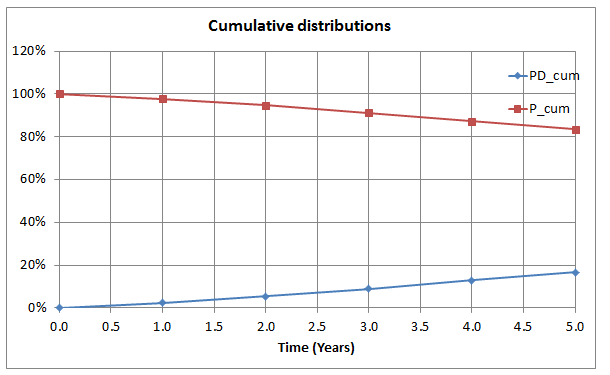
\includegraphics{../figs/cum_pd_psurv.PNG}
\caption{}
\end{figure}

    \subsection{Par 3 - Term Structure of Hazard
Rates}\label{par-3---term-structure-of-hazard-rates}

\begin{itemize}
\item
  The workings can be found in the tab \emph{part 2 \& 3} in the file
  above
\item
  From PsSurv \(P(0, T)\), the hazard rates can be calculated using the
  formula:
\end{itemize}

\[
\lambda_m = - \frac{1}{\Delta t} \ln \frac{P(0, t_m)}{P(0, t_{m-1})}
\]

The result is shown below - see excel workings for details

    \begin{longtable}[c]{@{}cc@{}}
\toprule
TIME (Years) & Lambda\tabularnewline
\midrule
\endhead
0.0 & -\tabularnewline
1.0 & 2.33519\%\tabularnewline
2.0 & 3.11599\%\tabularnewline
3.0 & 3.89258\%\tabularnewline
4.0 & 4.39091\%\tabularnewline
5.0 & 4.37817\%\tabularnewline
\bottomrule
\end{longtable}

    \begin{figure}[!htbp]
\centering
    \adjustimage{max size={0.6\linewidth}{0.9\paperheight}}{../figs/hazard_rates.PNG}
%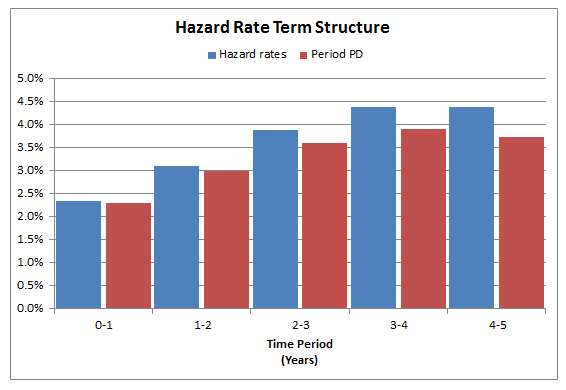
\includegraphics{../figs/hazard_rates.PNG}
\caption{}
\end{figure}

\newpage

    \begin{itemize}
\tightlist
\item
  Plotting the exponential pdf \(f(t) = \lambda e^{-\lambda t}\) for
  piecewise constant lambda the below plot is obtained. We note the
  instability at every tenor change, where we see `jumps' instead of a
  smooth continous function. In theory each tenor period will have it's
  own f(t) but given we only get the hazard rate for a given period, we
  see this reflected as well
\end{itemize}

    \begin{figure}[htbp]
\centering
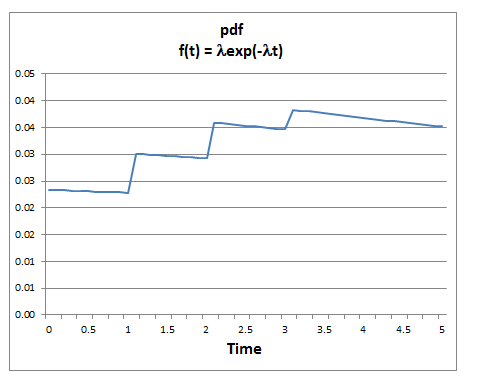
\includegraphics{../figs/pdf.PNG}
\caption{}
\end{figure}


    % Add a bibliography block to the postdoc
    
    
    
    \end{document}
